\documentclass[11pt,a4paper]{article}
\usepackage[T1]{fontenc}
\usepackage{lmodern}
\usepackage[utf8]{inputenc}
\usepackage[polish]{babel}
\usepackage{amsmath,amssymb,graphicx,booktabs,hyperref,listings}
\usepackage[normalem]{ulem}
\usepackage[margin=2.4cm]{geometry}
\hypersetup{colorlinks=true,urlcolor=blue,linkcolor=blue}
\lstset{basicstyle=\ttfamily\small,frame=single,breaklines=true}
\title{Rzut ukośny: te same elementy w LaTeX-u}
\author{Przykładowe rozwiązanie ćwiczenia}
\date{\today}
\begin{document}
\maketitle
\tableofcontents

\section{Opis}
\subsection{Cel}
Dokument pokazuje odpowiedniki elementów Markdown w LaTeX-u.
Badamy \textbf{ruch pocisku}, a dane opisujemy \textit{modelem}.
Zdanie \sout{Opór powietrza zawsze można pominąć} jest skreślone,
ponieważ zależy to od przyjętej dokładności.

\subsection{Założenia}
W modelu bez oporu prędkość początkowa wynosi $v_0$,
kąt wyrzutu to $\alpha$, a przyspieszenie grawitacyjne to $g$.
Są to trzy przykłady wzorów w tekście:
$v_x=v_0\cos\alpha$, $v_y(0)=v_0\sin\alpha$ oraz
$T=2v_0\sin\alpha/g$.

\section{Listy i checklista}
\begin{itemize}
  \item Ustal układ współrzędnych.
  \item Podaj jednostki SI.
\end{itemize}
\begin{enumerate}
  \item Zapisz warunki początkowe.
  \item Oblicz tor i zasięg.
  \item Porównaj wynik z wykresem.
\end{enumerate}
\noindent$\boxtimes$ Model bez oporu opisany \qquad
$\boxtimes$ Wzory sprawdzone \qquad
$\square$ Pomiar doświadczalny wykonany

\section{Wzory, tabela i wykres}
Trzy osobne wzory matematyczne:
\begin{equation}
x(t)=v_0\cos\alpha\,t .
\end{equation}
\begin{equation}
y(t)=v_0\sin\alpha\,t-\frac{gt^2}{2}.
\end{equation}
\begin{equation}
R=\frac{v_0^2\sin(2\alpha)}{g}.
\end{equation}
\begin{center}
\begin{tabular}{lll}
\toprule
Wielkość & Symbol & Jednostka \\
\midrule
Prędkość początkowa & $v_0$ & $\mathrm{m\,s^{-1}}$ \\
Czas lotu & $T$ & $\mathrm{s}$ \\
Zasięg & $R$ & $\mathrm{m}$ \\
\bottomrule
\end{tabular}
\end{center}

\begin{figure}[htbp]
\centering
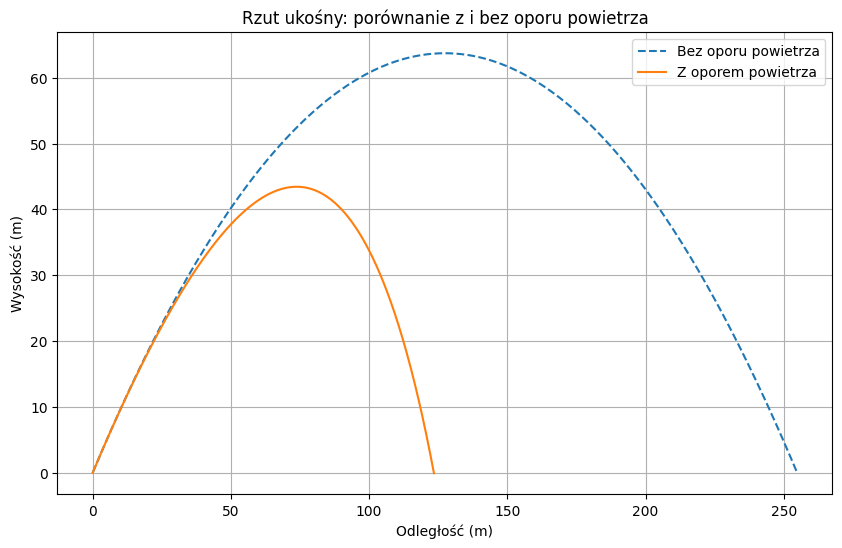
\includegraphics[width=.82\linewidth]{wykres.png}
\caption{Przykładowy wykres porównujący tor bez oporu i z oporem powietrza.
Grafika pochodzi z dostarczonego folderu \texttt{assets/05\_sol\_latex/02\_start}.}
\end{figure}

\section{Link i kod}
Odnośnik: \href{https://colab.research.google.com}{Google Colab}.
Krótki fragment Pythona obliczający zasięg modelu bez oporu:
\begin{lstlisting}[language=Python]
import math
v0, alpha, g = 50.0, math.radians(45), 9.81
R = v0**2 * math.sin(2 * alpha) / g
print(f"Zasieg: {R:.2f} m")
\end{lstlisting}
\end{document}
